Now that you have managed to successfully complete a GITM run you've found yourself with a bunch of output files.  All of the GITM output is in mks units and this data is contained within several files located in the {\tt UA/data} directory, as was previously discussed in Chapter~\ref{quickstart.ch} Section~\ref{post_process.sec}.  You will have found yourself with several {\tt iriOut\_*.dat} files, a {\tt log*.dat} file, and many {\tt .bin} files in whichever formats you specified in SAVEPLOT (see Chapter~\ref{input.ch} Section~\ref{def_out.sec}).  The {\tt iriOut\_*.dat} files are required by the IRI model and not typically used when analyzing the outcome of the GITM run.

The log file provides useful information about the run, such as whether a restart was performed, which physical processes were used, and a list of the universal time, time-step, neutral temperature ranges (T), solar and geomagnetic indices, and the neutral velocity (VV) ranges for each iteration.  This file can be very useful when sharing runs with other users, when revisiting an old run, or merely ensuring that GITM performed as expected.  An example log file is provided below:

\begin{verbatim}
## Inputs from UAM.in
# Resart= F
# Eddy coef:   100.000 Eddy P0:     0.020 Eddy P1:     0.003 Eddy Scaling:     1.000
# Statistical Models Only:  F Apex:  T
# EUV Data:  TFile: 
fismflux.dat                                                                                        
# AMIE: none           
none                                                                                                
# Solar Heating:  T Joule Heating:  T Auroral Heating:  T
# NO Cooling:  T O Cooling:  T
# Conduction:  T Turbulent Conduction:  T Updated Turbulent Conduction:  T
# Pressure Grad:  T Ion Drag:  T Neutral Drag:  T
# Viscosity:  T Coriolis:  T Gravity:  T
# Ion Chemistry:  T Ion Advection:  T Neutral Chemistry:  T
 
#START
   iStep yyyy mm dd hh mm ss  ms      dt min(T) max(T)...
   ...mean(T) min(VV) max(VV) mean(VV) F107 F107A By Bz Vx...
   ...HP HPn HPs SubsolarLon SubsolarLat SubsolarVTEC
       2 2011  9 23  0  0  2 297  2.2979  168.75192  1062.87354...
       ...933.09984 -48.19362    524.93645  1.01910 159.3 127.9 -4.6  0.5 406.9...
       ...11.1 14.4  15.5  3.14145  -0.37655  45.73188
       .
       .
       .
\end{verbatim}

The 3DALL output binary files can contain the following atmospheric quantities:

\begin{itemize}
\item[]{\bf Altitude:} Altitude from the surface of the planet (m)
\item[]{\bf Ar:} Argon density (m$^{-3}$)
\item[]{\bf Ar Mixing Ratio:} Argon mixing ratio
\item[]{\bf CH4 Mixing Ratio:} Methane mixing ratio
\item[]{\bf Conduction:} Heat conduction
\item[]{\bf EuvHeating:} EUV Heating rate
\item[]{\bf H:} Hydrogen density (m$^{-3}$)
\item[]{\bf H!U+!N:} H$^+$ density (m$^{-3}$)
\item[]{\bf H2 Mixing Ratio:} Molecular Hydrogen mixing ratio
\item[]{\bf HCN Mixing Ratio:} Hydrogen Cyanide mixing ratio
\item[]{\bf He:} Helium density (m$^{-3}$)
\item[]{\bf He!U+!N:} He$^+$ density (m$^{-3}$)
\item[]{\bf Heaing Efficiency:} Heating efficiency
\item[]{\bf Heat Balance Total:} Heat balance total
\item[]{\bf Latitude:} Geographic latitude (degrees)
\item[]{\bf Longitude:} Geographic longitude (degrees)
\item[]{\bf N!D2!N:} N$_2$ density (m$^{-3}$)
\item[]{\bf N!D2!U+!N:} N$_2^+$ density (m$^{-3}$) 
\item[]{\bf N!U+!N:} N$^+$ density (m$^{-3}$)
\item[]{\bf N(!U2!ND):} N($^2$D) density (m$^{-3}$)
\item[]{\bf N(!U2!NP):} N($^2$P) density (m$^{-3}$)
\item[]{\bf N(!U4!NS):} N($^4$S) density (m$^{-3}$)
\item[]{\bf N2 Mixing Ratio:} Molecular nitrogen mixing ratio
\item[]{\bf NO:} Nitrious Oxide density (m$^{-3}$)
\item[]{\bf NO!U+!N:} NO$^+$ density (m$^{-3}$)
\item[]{\bf O!D2!N:} O$_2$ density (m$^{-3}$)
\item[]{\bf O!D2!U+!N:} O$_2^+$ density (m$^{-3}$)
\item[]{\bf O(!U1!ND):} O($^1$D) density (m$^{-3}$)
\item[]{\bf O(!U2!ND)!U+!N:} O($^2$D) density (m$^{-3}$)
\item[]{\bf O(!U2!NP)!U+!N:} O($^2$P) density (m$^{-3}$)
\item[]{\bf O(!U3!NP):} O($^3$P) density (m$^{-3}$)
\item[]{\bf O\_4SP\_!U+!N:} O($_4$SP)$^+$ density (m$^{-3}$)
\item[]{\bf RadCooling:} Radiative Cooling rate
\item[]{\bf Rho:} Neutral density (m$^{-3}$)
\item[]{\bf Temperature:} Neutral temperature (K)
\item[]{\bf V!Di!N (east):} Ion velocity towards geographic East (m s$^{-1}$)
\item[]{\bf V!Di!N (north):} Ion velocity towards geographic North (m s$^{-1}$) 
\item[]{\bf V!Di!N (up):} Vertical ion velocity (m s$^{-1}$)
\item[]{\bf V!Dn!N (east):} Neutral velocity towards geographic East (m s$^{-1}$)
\item[]{\bf V!Dn!N (north):} Neutral velocity towards geographic North (m s$^{-1}$)
\item[]{\bf V!Dn!N (up):} Vertical neutral velocity (m s$^{-1}$)
\item[]{\bf V!Dn!N (up,N!D2!N):} Vertical N$_2$ velocity (m s$^{-1}$)
\item[]{\bf V!Dn!N (up,N(!U4!NS)):} Vertical N($^4$S) velocity (m s$^{-1}$)
\item[]{\bf V!Dn!N (up,NO):} Vertical NO velocity (m s$^{-1}$)
\item[]{\bf V!Dn!N (up,O!D2!N):} Vertical O$_2$ velocity (m s$^{-1}$)
\item[]{\bf V!Dn!N (up,O(!U3!NP)):} Vertical O($^3$P) velocity (m s$^{-1}$)
\item[]{\bf e-:} electron density (m$^{-3}$)
\item[]{\bf eTemperature:} electron temperature (K)
\item[]{\bf iTemperature:} ion temperature (K)
\item[]{\bf time:} Universal time
\end{itemize}

There are many routines available to process and analyze the GITM binary files.  The majority of these routines are written in IDL and are available in the {\tt srcIDL} directory within the GITM model directory.  Currently 50 routines have been saved in this directory and more are under development.  Alternatively, python routines are currently being developed and these are located in the {\tt srcPython} directory.  Please not that when using the IDL reader the universal time is read in as epoch seconds from January 1, 1965 00:00 UT, while when using the python reader, the time is imported as a datetime object.

\section{IDL}
\label{idl.sec}

Here is an complete list with some description of the IDL processing and visualization routines currently available.  Please feel free to update this section for other GITM users when you CVS your vetted GITM processing routines.
 
\subsubsection{gitm\_read\_bin}

This is a routine to read a GITM bin file into IDL.  This is great when you want to get a handle on the data and experiment with different visualization methods.

\subsubsection{thermo\_plotsat}

This is the most commonly used routine to plot the 1D GITM results.  It can also be used to plot satellite files and other 1D simulations.  It is relatively straight forward to use, but experimentation can be help.  This is an actual program, so you have to {\tt .run} it.

\subsubsection{thermo\_gui}

This is a someone simplistic graphical user interface code for plotting 3D results.  The filename has to be entered manually in the upper left.  You then have to press the button for loading the file.  Variables appear on the left side, and you can select which one you want to plot.  You then select which of the available planes you would like to look at (lat/lon, lat/alt, or lon/alt) or scroll through the options.  This interface allows you to add wind vectors, plot in polar coordinates, and plot the log of the variable.

\subsubsection{thermo\_batch\_new}

This code will let you look at at 3D files exactly the same way as thermo\_gui, but is all scripted.  There are a few features that this has that thermo\_batch doesn't have:

\begin{enumerate}
%\setlength{\itemsep}{-3in}
	\item You can use wildcards for the file name, so that a list of files can be read.  The postscript file names created for each figure will be differentiated by appending numbers sequentially so that no figures are overwritten.
	\item When plotting a lat/alt plane, you can do a zonal average. 
	\item You can do a global average.
\end{enumerate}

\subsubsection{thermo\_plotter}

All of the above plotting codes will only plot one plot per page.  This code will plot many more than one plot per page.  You can plot multiple variables on the same page, or multiple files with the same variable, or both.

\subsubsection{Other IDL Routines}

Please feel free to provide a description of these routines so that GITM users do not waste their time rewriting code that already exists.

\begin{multicols}{3}
\begin{itemize}
\item{\bf ask}
\item{\bf c\_a\_to\_r}
\item{\bf c\_a\_to\_s}
\item{\bf chopr}
\item{\bf closedevice}
\item{\bf c\_r\_to\_a}
\item{\bf c\_s\_to\_a}
\item{\bf get\_position}
\item{\bf makect}
\item{\bf mklower}
\item{\bf mm}
\item{\bf plotct}
\item{\bf plotdumb}
\item{\bf plotmlt}
\item{\bf pos\_space}
\item{\bf read\_thermosphere\_file}
\item{\bf setdevice}
\item{\bf thermo\_batch}
\item{\bf thermo\_calcforce}
\item{\bf thermo\_champ}
\item{\bf thermo\_compare}
\item{\bf thermo\_compare\_time}
\item{\bf thermo\_convert\_champfiles}
\item{\bf thermo\_guvi}
\item{\bf thermo\_magequator}
\item{\bf thermo\_make\_summary}
\item{\bf thermo\_mkguvisat}
\item{\bf thermo\_mksatsave}
\item{\bf thermo\_mksave}
\item{\bf thermo\_mktec}
\item{\bf thermo\_on2}
\item{\bf thermo\_plotdist}
\item{\bf thermo\_plotlog}
\item{\bf thermo\_plot\_new}
\item{\bf thermo\_plot}
\item{\bf thermo\_plotsat2}
\item{\bf thermo\_plotsat\_constalt\_ON2}
\item{\bf thermo\_plotsat\_constalt}
\item{\bf thermo\_plotvectors}
\item{\bf thermo\_readsat}
\item{\bf thermo\_sigma}
\item{\bf thermo\_superposed}
\item{\bf thermo\_tec}
\item{\bf thermo\_temp}
\item{\bf tostr}
\end{itemize}
\end{multicols}

\section{Python}
\label{python.sec}

This section provides a complete list of the vetted GITM python routines.  These routines require that you use PyBats, a module included in SpacePy.  This is a library developed for space physics applications by the scientists at Los Alamos and can be downloaded for free at: 
{\tt http://spacepy.lanl.gov}

Another library, Basemap, is required for certain plotting routines.  Basemap is a part of the Matplotlib Toolkit and can be installed using Fink, Macports, or downloaded at:
{\tt http://matplotlib.org/basemap/}

Python scripts that create movies rely on external programs to do so.  The scripts included here use FFmpeg, which can be installed using Fink, Macports, or downloaded at: {\tt http://http://www.ffmpeg.org/}

If you have questions about these routines or are at the University of Michigan and want to start using Python, Dr. Welling is the man to see.  The source code behind the PyBats GITM routines are also located in {\tt GITM2/srcPython}.

The following programs include the vetted python routines.  The examples shown are meant to be run in ipython, an interactive command-line interface for python.  The terminal window that is running ipython should be located in the {\tt GITM2/srcPython} directory.  The test file for the example code is one of the files output after running the default {\tt UAM.in} file.

\subsubsection{gitm.py}

GITM is a PyBats submodule that handles input and output from GITM.  It can be helpful for those wishing to write their own GITM processing routines but doesn't contain any analysis or visualization routines. 

Once you have downloaded and installed Spacepy, the gitm submodule can be accessed via {\tt import spacepy.pybats.gitm}.  This module contains the following routines:

\begin{itemize}
\item[]{\bf GitmBin: } A data class and routine to load a GITM output bin file.  Geographic position in degrees and local time are also added to the output.  Once a 3DION file is associated with the output GITM structure (by assigning a filename to the attribute `ionfile'), the ion velocity can be computed in magnetic field coordinates.
\item[]{\bf PbData: } The base class for all PyBats data container classes.  Used to hold the GITM data read in using GitmBin
\item[]{\bf dt: } A shortcut for datetime.
\item[]{\bf np: } A shortcut for numpy.
\item[]{\bf dmarray: } A shortcut for data arrays.  Used in many of the data container classes defined in PbData.
\end{itemize}

You can load a GITM binary file by entering the following commands.  Comments are preceded by a `\#'.

\begin{verbatim}
In [1]: import spacepy
In [2]: import gitm # Load the local version of gitm.py, which may be more up-to-date
In [3]: gdata = gitm.GitmBin(`3DALL_t021124_000000.bin') # example binary file
In [4]: gdata.attrs
Out[4]:
{`endian': `big',
 `file': `3DALL_t021124_000000.bin',
 `nAlt': 54,
 `nLat': 22,
 `nLon': 22,
 `nVars': 39,
 `version': 3.13}
\end{verbatim}

\subsubsection{gitm\_time.py}

gitm\_time has not yet been incorporated into PyBats, as it is actively being developed.   This module contains the following routines:

\begin{itemize}
\item[]{\bf GitmTime: } A data class and routine to load multiple GITM output binaries into a structure that includes a universal time (UT) dimension.  All data types and attributes provided by GitmBin are provided in this data class.
\item[]{\bf load\_multiple\_gitm\_bin: } A routine to load a list of GITM output binary files into GitmBin data structures.  The output is a list of the GitmBin structures, where each element in the list contains the data from a GITM output binary.
\end{itemize}

You can load multiple GITM binary files into a data structure with UT dependence by entering the following commands.  Commands outside of ipython are preceded by a `\$'.  Again, the output files used are produced by running the default {\tt UAM.in} file.

\begin{verbatim}
$ ls 3DALL_t021124_000* > test.list
$ ipython
In [1]: import spacepy
In [2]: import gitm # Load the local version of gitm.py, which may be more up-to-date
In [3]: import gitm_time as gt
In [4]: gtdata = gt.GitmTime(`test.list')
In [5]: print gtdata['time'][:]
[datetime.datetime(2002, 11, 24, 0, 0)
 datetime.datetime(2002, 11, 24, 0, 5)]
In [6]: print gtdata['dLon'][0,:,10,27]
[ -30.  -10.   10.   30.   50.   70.   90.  110.  130.  150.  170.  190.
  210.  230.  250.  270.  290.  310.  330.  350.  370.  390.]
In [7]: print gtdata['dLat'][0,10,:,27]
[-105.  -95.  -85.  -75.  -65.  -55.  -45.  -35.  -25.  -15.   -5.    5.
   15.   25.   35.   45.   55.   65.   75.   85.   95.  105.]
In [8]: print gtdata['Altitude'][0,10,10,:]
[  96660.90047544   98330.45023772  100000.          101669.54976228
  103348.94180562  105050.15497984  106788.53042153  108584.61276626
  110467.61429397  112482.48190265  114698.91401856  117219.51380361
  120200.6752566   123855.40706002  128245.43857411  133349.83464183
  139220.53740507  145894.02746965  153389.42319611  161708.33330952
  170836.59866663  180746.14929878  191399.58798926  202753.75931196
  214763.18484817  227382.89781152  240569.83529396  254283.5502381
  268486.11667059  283141.61144778  298215.46358093  313673.89525175
  329480.19139848  345605.83193525  362018.21624294  378685.73558327
  395578.19775965  412667.22510966  429926.74623085  447332.78448625
  464864.02590453  482501.63589793  500229.1662886   518032.39821451
  535899.14534895  553819.03817939  571783.3052721   589784.56266012
  607816.61836022  625874.29578468  643953.27746286  662049.96890339
  680161.38144647  698272.79398955]
\end{verbatim}

\subsubsection{gitm\_plot\_rout.py}

Common routines used to format and analyze GITM data.

\begin{itemize}
\item[]{{\bf add\_colorbar:}  Add a color bar to a contour plot.  This routine does not depend on SpacePy.}
\item[]{{\bf center\_polar\_cap:}  Adjust radial coordinates to produce a centered polar plot.  Necessary for the northern hemisphere, where polar plots assume the radial (latitude) coordinates should be centered at zero instead of 90$^\circ$.  This routine does not depend on SpacePy.}
\item[]{{\bf find\_data\_limits:}  Find the upper and lower limits for a specified data key in a list of GITM data structures at a specified location (either single indices or the entire range are permitted for latitude, longitude, and altitude).}
\item[]{{\bf find\_data\_limits\_irange:}  Find the upper and lower limits for a specified data key in a list of GITM data structures at a specified location range (upper and lower limits or the entire range are permitted for latitude, longitude, and altitude).}
\item[]{{\bf localtime\_to\_glon:}  Find the longitude at a specified universal time and local time.}
\item[]{{\bf find\_lon\_lat\_index:}  Find the indexes for the location closest to a specified latitude and longitude.}
\item[]{{\bf retrieve\_key\_from\_web\_name:}  Find a data key given a website-friendly version of data key names.}
\item[]{{\bf find\_alt\_index:} Find the index closest to the specified altitude.  Altitude may be specified in km or m.}
\end{itemize}

This example shows how the index for a specified altitude can be found.  Note that GITM saves altitude in meters.

\begin{verbatim}
In [1]: import spacepy
In [2]: import gitm
In [3]: import gitm_plot_rout as gpr
In [4]: gdata = gitm.GitmBin(`3DALL_t021124_000000.bin')
In [5]: ialt = gpr.find_alt_index(gdata, 10, 10, 250.0, "km")
In [6]: print ialt, gdata['Altitude'][10,10,ialt]
27 254283.550238
\end{verbatim}

\subsubsection{gitm\_3D\_global\_plots.py}

Routines to build and output GITM output variable contour plots over a geographic range.  Several different standard plot formats are available, and routines useful for creating custom figures are also included.

\begin{itemize}
\item[]{{\bf plot\_single\_3D\_image:}  This is a basic visualization routine that creates a filled contour plot of a single output variable from a GITM 3D at a specified altitude or 2D bin file.  The output variable is plotted as a function of latitude and longitude over the entire globe, though the latitude range may be limited.  The output plot may be polar or rectangular and a map of the Earth's continental boundaries may also be included in the output figure.  Sample output of the electron temperature is shown in figure~\ref{gitm_3D_global_plots.fig}~(a) and~(b).}
\item[]{{\bf plot\_single\_nsglobal\_3D\_image:}  A quick way to examine GITM output at both poles.  This routine creates two polar contour plots centered at the geographic northern and southern poles for a single output variable from a GITM 3D at a specified altitude or 2D bin file.  The equatorial and polar latitude boundaries may both be specified, though they cannot change between hemispheres.  The Earth's continental boundaries may also be included in the output figure.  Sample output of the electron temperature is shown in figure~\ref{gitm_3D_global_plots.fig}~(c)}
\item[]{{\bf plot\_global\_3D\_snapshot:}  A snapshot of a single GITM output over the entire globe.  This routine creates two polar contour plots centered at the geographic northern and southern poles and extending to 45$^\circ$ and a single rectangular plot containing the mid- and low-latitudes for a single output variable from a GITM 3D at a specified altitude or 2D bin file.  The Earth's continental boundaries may also be included in the output figure.  Sample output of the electron temperature is shown in figure~\ref{gitm_3D_global_plots.fig}~(d)}
\item[]{{\bf plot\_mult\_3D\_slices:}  This routine creates a single plot containing multiple global contours of a GITM output variable from a 3D or 2D bin file at a list of specified altitudes.  These plots may be either polar or rectangular, with or without continental outlines, and within a specified latitude range.  Sample output of the electron temperature is shown in figure~\ref{gitm_3D_mult_plots.fig}.}
\item[]{{\bf plot\_rectangular\_3D\_global:} This routine plots a single rectangular filled contour for a GITM output variable at a specified altitude index as a function of latitude and longitude.  Title, colorbar, and continental outlines are optional.  A handle to the contour plot is returned to allow the output to be further manipulated depending on what other subplots are included in the output figure.} 
\item[]{{\bf plot\_polar\_3D\_global:} This routine plots a single polar filled contour for a GITM output variable at a specified altitude index as a function of latitude and longitude.  Title, colorbar, and continental outlines are optional.  A handle to the contour plot is returned to allow the output to be further manipulated depending on what other subplots are included in the output figure.  The longitude at the top of the plot may also be specified, this allows one to ensure a specific local time is always located at the top of the dial using a routine like {\bf localtime\_to\_glon}.} 
\end{itemize}

\begin{figure}
\begin{center}
\subfigure[]{
\noindent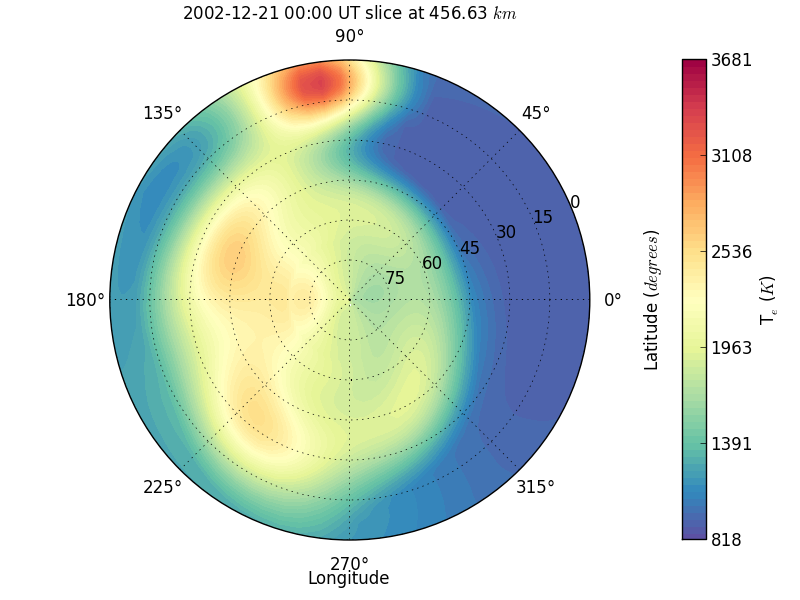
\includegraphics[width=.45 \textwidth]{Figures/plot_single_3D_image_polar.png}
}
\subfigure[]{
\noindent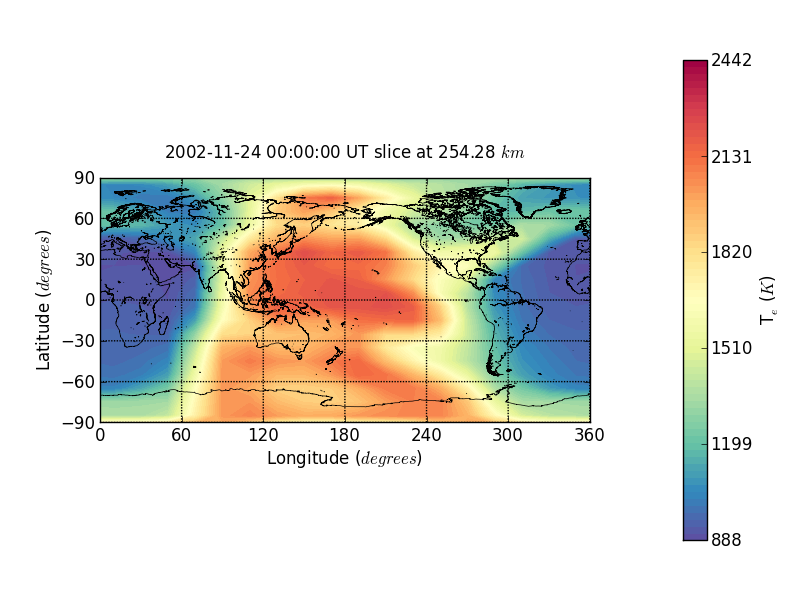
\includegraphics[width=.45 \textwidth]{Figures/plot_single_3D_image_rect.png}
}
\subfigure[]{
\noindent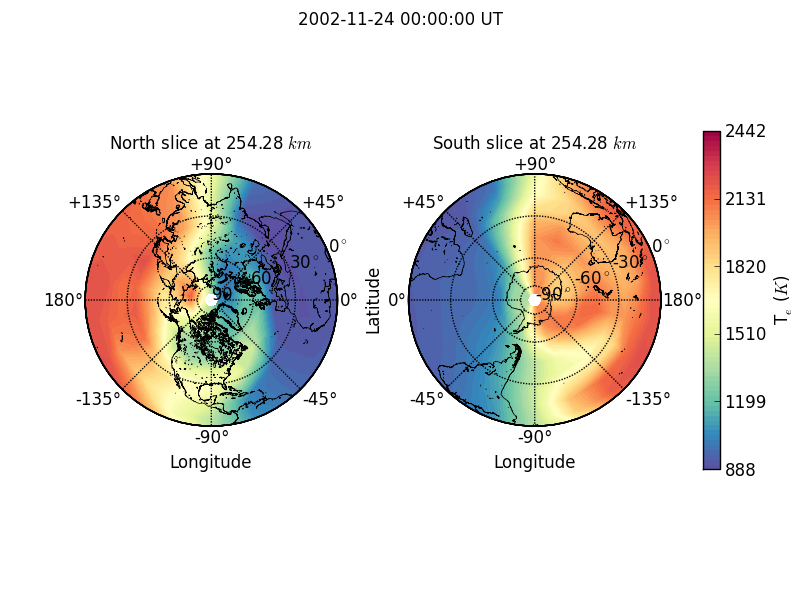
\includegraphics[width=.45 \textwidth]{Figures/plot_single_nsglobal_3D_image.png}
}
\subfigure[]{
\noindent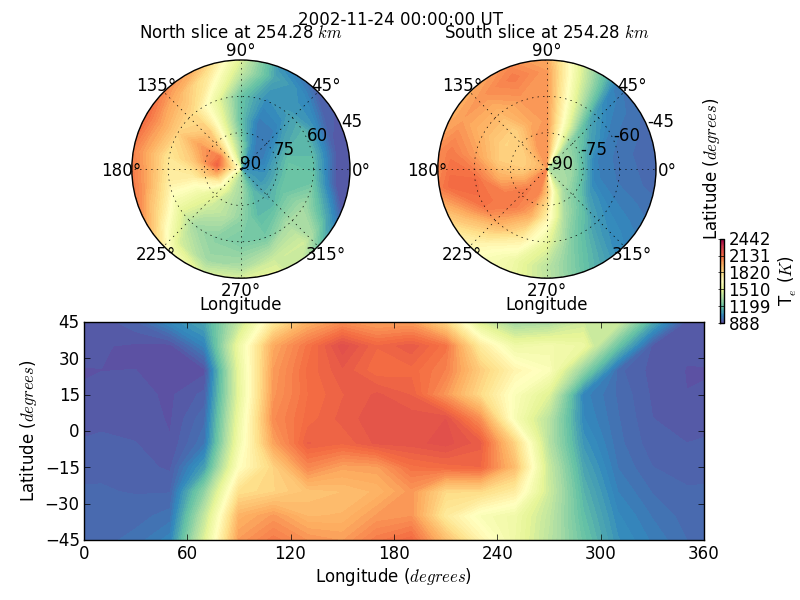
\includegraphics[width=.45 \textwidth]{Figures/plot_global_3D_snapshot.png}
}
\caption{GITM electron temperature at 456.63 $km$ altitude for: (a) northern latitudes, (b) over the entire globe, (c) over the entire globe, as viewed from the poles, and (d) as a global snapshot.}
\label{gitm_3D_global_plots.fig}
\end{center}
\end{figure}

\begin{figure}
\begin{center}
\subfigure[]{
\noindent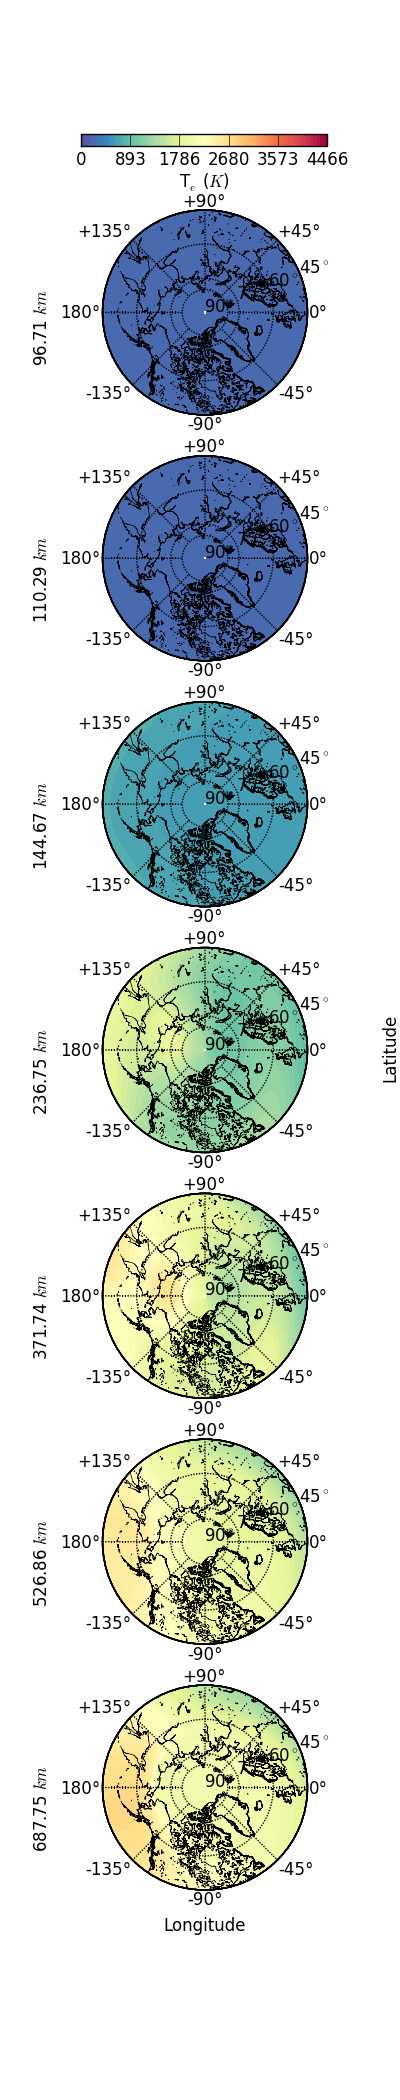
\includegraphics[height=.9 \textheight]{Figures/plot_mult_3D_slices_polar.png}
}
\subfigure[]{
\noindent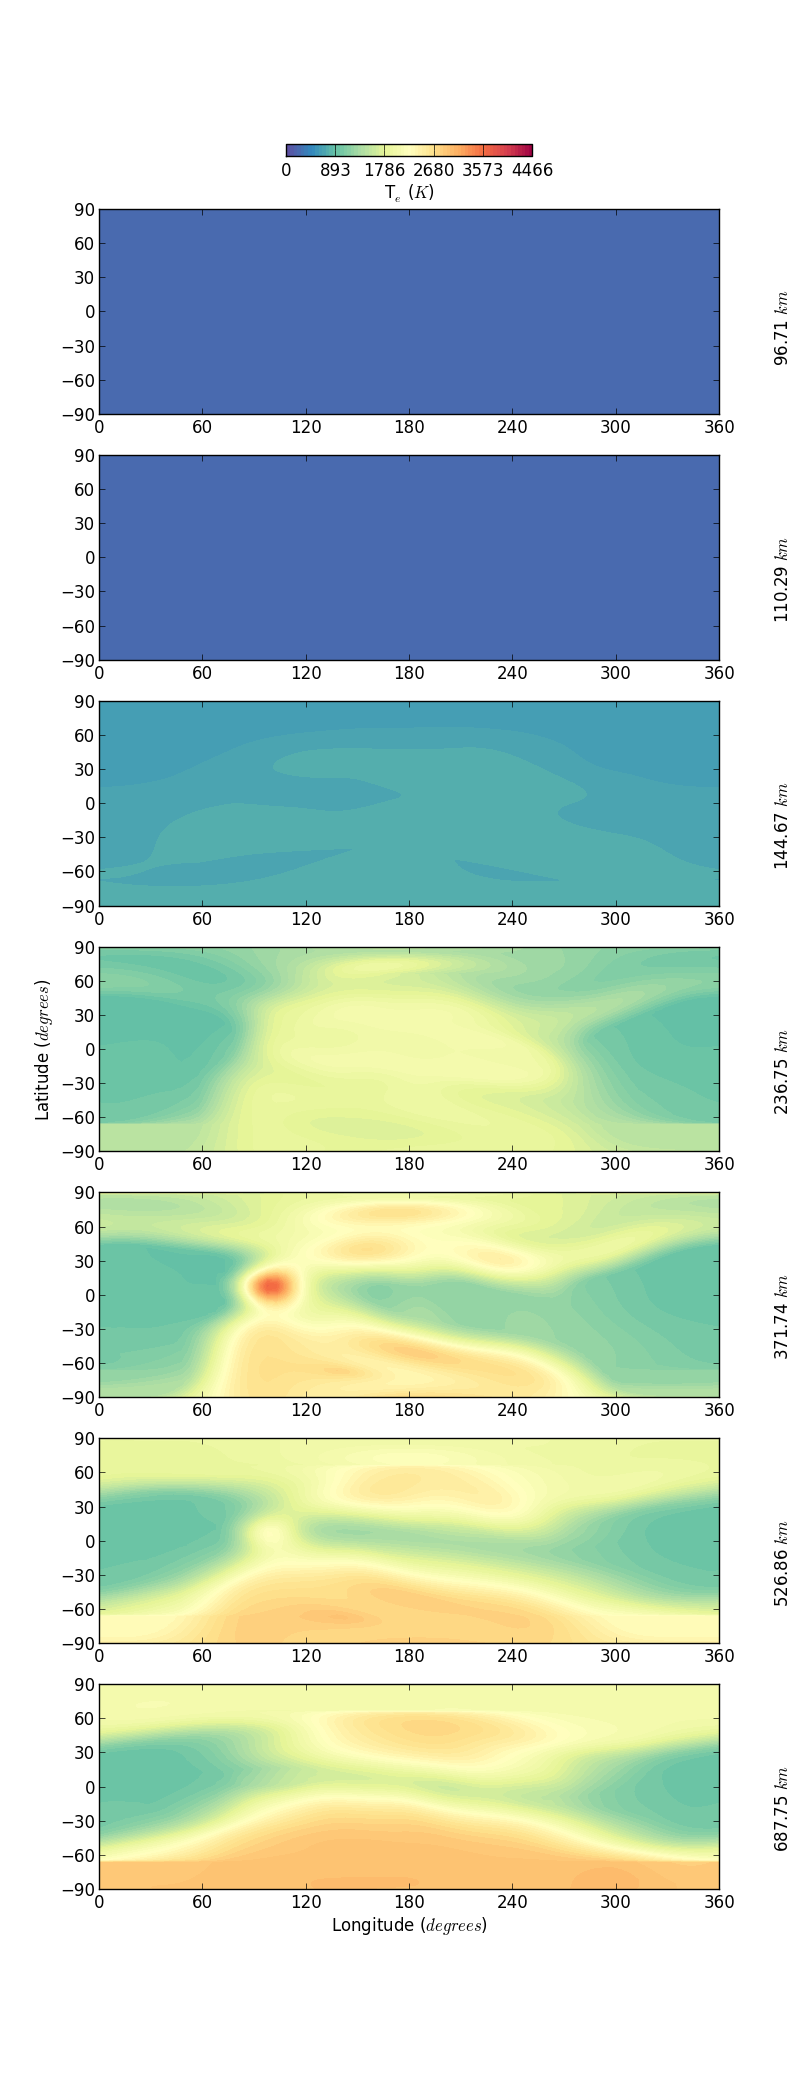
\includegraphics[height=.9 \textheight]{Figures/plot_mult_3D_slices_rect.png}
}
\caption{GITM electron temperature at seven altitude slices for (a) northern latitudes and (b) the entire globe.}
\label{gitm_3D_mult_plots.fig}
\end{center}
\end{figure}

\subsubsection{gitm\_alt\_plots.py}

Routines to build and output GITM output variable linear and contour plots over an altitude range.  Several different standard plot formats are available, and routines useful for creating custom figures are also included.

\begin{itemize}
\item[]{{\bf plot\_single\_alt\_image:}  Creates a single linear or contour altitude plot.}
\item[]{{\bf plot\_mult\_alt\_image:}  Creates a figure with multiple linear or contour altitude plots.}
\item[]{{\bf plot\_alt\_slices:}  Creates a figure with a contour plot showing the altitude dependence of a quantity as a function of latitude or longitude with several linear altitude slices at specified locations.  An example is shown in figure~\ref{gitm_alt_slices.fig}}
\item[]{{\bf plot\_linear\_alt:}  Plots the the linear altitude dependence of a quantity, with altitude on the y-axis.}
\item[]{{\bf plot\_3D\_alt:}  Plots the altitude dependence of a quantity as the function of another spatiotemporal coordinate with the spatiotemporal coordinate on the x-axis, altitude on the y-axis, and the desired quantity as a color contour.}
\end{itemize}

\begin{figure}
\begin{center}
\noindent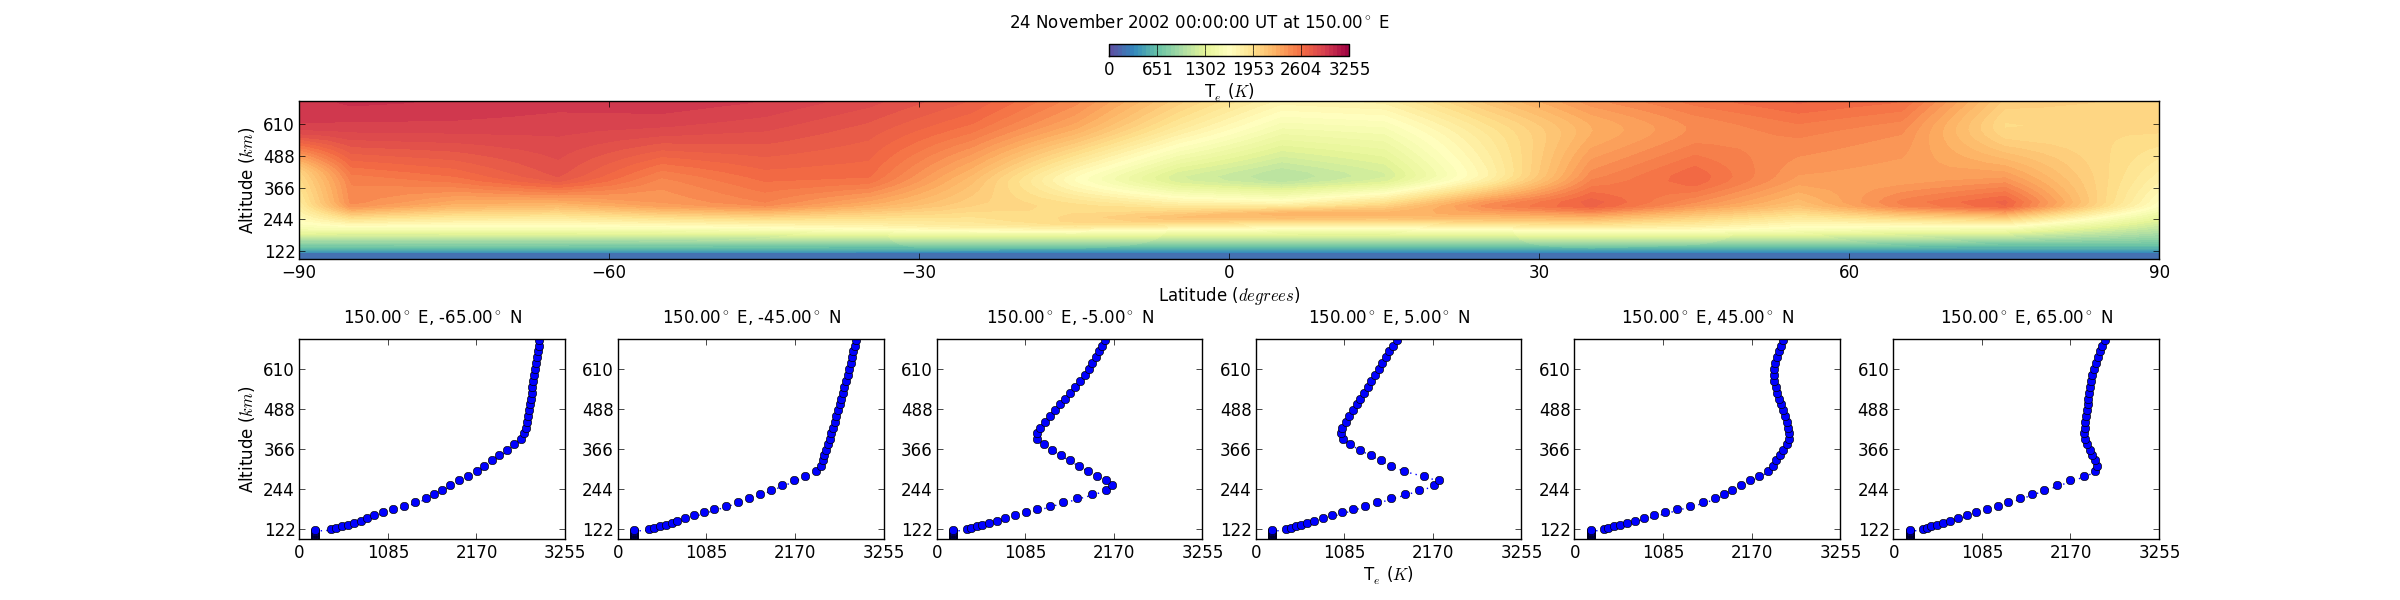
\includegraphics[width=\textwidth]{Figures/gitm_alt_slice_test_Te.png}
\caption{GITM electron temperature at a constant longitude with six latitude slices.}
\label{gitm_alt_slices.fig}
\end{center}
\end{figure}

\subsubsection{gitm\_movie\_script.py}

This is a python script that can be run either from ipython using the command {\tt run gitm\_movie\_script.py} or the command line using the command {\tt python gitm\_movie\_script.py}.  Input to this program is prompted interactively, and includes:

\begin{itemize}
\item{{\tt Ordered list of GITM binary files:}  A list of GITM binary files in chronological order (or whatever other order the movie should be played in).}
\item{{\tt GITM plot type (rectangular, polar, nspolar, snapshot):}  The keyword for the desired plot type.  These are the plot types shown in figure~\ref{gitm_3D_global_plots.fig}, where polar corresponds to panel (a), rectangular to panel (b), nspolar to panel (c), and snapshot to panel (d).}
\item{At this point, the routine enters a while-loop to allow multiple movies to be made for the same list of GITM binary files}
	\begin{itemize}
	\item{{\tt GITM key to plot on z axis (eg Temperature):} The data key corresponding to the data type to plot on the z axis.  A list of data keys can be found by typing `{\tt gdata.keys()}' into ipython after loading one of the listed GITM binaries.}
	\item{{\tt Altitude to plot z value at (eg 250):} Altitude to plot, may be specified in km or m.  For 2D parameters, a value must be entered, but doesn't matter.}
	\item{{\tt Units of altitude (km or m):} Units of altitude entered above.}
	\item{{\tt Use map of Earth? (empty for False):} Enter any value to include a Basemap plot of the earth, enter a carriage return to exclude the map.}
	\item{The latitude limits needed depend on the plot type}
		\begin{itemize}
		\item{{\bf for nspolar}  {\tt Polar latitude limit (degrees):} Specify the polar latitude limit (positive, same for both hemispheres).}
		\item{{\bf for nspolar} {\tt Equatorial latitude limit (degrees):} Specify the equatorial latitude limit (positive, same for both hemispheres).}
		\item{{\bf snapshot} {\tt Polar latitude limit (degrees):} Specify the polar latitude limit (positive, same for both hemispheres).}
		\item{{\bf polar/rectangular} {\tt Northern latitude limit (degrees):} Specify the northernmost latitude (may be negative).}
     	   	\item{{\bf polar/rectangular} {\tt Southern latitude limit (degrees):} Specify the southernmost latitude (must be smaller/more negative than the northernmost limit)}
		\end{itemize}
		
    \item{{\tt Load another z axis key? (empty for False):} Enter any value to include another movie or, enter a carriage return finish.}
    \end{itemize}
\end{itemize}

With this information, movies with appropriate z-variable ranges will be plot as .png files and combined into a movie using FFmpeg.  The image and movie files will be named using the plot type, z parameter, and altitude to distinguish them.







